\documentclass[conference]{IEEEtran}
\IEEEoverridecommandlockouts
\usepackage{cite}
\usepackage{amsmath,amssymb,amsfonts}
\usepackage{algorithmicx}
\usepackage{algcompatible}
\usepackage{graphicx}
\usepackage{textcomp}
\usepackage{xcolor}
\usepackage{hyperref}
\usepackage{algorithm}
\usepackage{algpseudocode}
\usepackage{caption}
\def\BibTeX{{\rm B\kern-.05em{\sc i\kern-.025em b}\kern-.08em
    T\kern-.1667em\lower.7ex\hbox{E}\kern-.125emX}}
\begin{document}

% ─────────────────────────────────────────────────────────────────
% 1. TITLE (Centered, Bold)
% ─────────────────────────────────────────────────────────────────
\title{\textbf{Generalized Tic-Tac-Toe Solver Using Two Different Approaches}}

% ─────────────────────────────────────────────────────────────────
% 2. AUTHOR NAMES & AFFILIATIONS
% ─────────────────────────────────────────────────────────────────
\author{
\IEEEauthorblockN{Mahmoud Sayed}
\IEEEauthorblockA{\textit{Faculty of Computer Science} \\
\textit{Misr International University}\\
\href{mailto:mahmoud2406330@miuegypt.edu.eg}{\textit{mahmoud2406330@miuegypt.edu.eg}}}
\and
\IEEEauthorblockN{Salma Mahmoud}
\IEEEauthorblockA{\textit{Faculty of Computer Science} \\
\textit{Misr International University}\\
\href{mailto:salma2408613@miuegypt.edu.eg}{\textit{salma2408613@miuegypt.edu.eg}}}
\and
\IEEEauthorblockN{Razan Ismail}
\IEEEauthorblockA{\textit{Faculty of Computer Science} \\
\textit{Misr International University}\\
\href{mailto:razan2404368@miuegypt.edu.eg}{\textit{razan2404368@miuegypt.edu.eg}}}
\and
\IEEEauthorblockN{Mina Samaan}
\IEEEauthorblockA{\textit{Faculty of Computer Science} \\
\textit{Misr International University}\\
\href{mailto:mina2404830@miuegypt.edu.eg}{\textit{mina2404830@miuegypt.edu.eg}}}
\and
\IEEEauthorblockN{Sama Mohamed}
\IEEEauthorblockA{\textit{Faculty of Computer Science} \\
\textit{Misr International University}\\
\href{mailto:sama2400293@miuegypt.edu.eg}{\textit{sama2400293@miuegypt.edu.eg}}}
\and
\IEEEauthorblockN{Dr. Ashraf Abdel Raouf}
\IEEEauthorblockA{\textit{Professor in Computer Science} \\
\textit{Misr International University}\\
\href{mailto:ashraf.raouf@miuegypt.edu.eg}{\textit{ashraf.raouf@miuegypt.edu.eg}}}
}

\maketitle

% ─────────────────────────────────────────────────────────────────
% 3. ABSTRACT (150-250 words, one paragraph, no citations)
% ─────────────────────────────────────────────────────────────────
\begin{abstract}
The generalized Tic-Tac-Toe problem requires computing the optimal move
on an $N \times N$ board with a $K$-in-a-row win condition, modeled as
a two-player zero-sum adversarial game. This study compares two
algorithmic strategies: a pure brute-force Minimax recursion and a
memoized Minimax using dynamic programming (DP). Both approaches are
implemented in C++, their structures are described, their computational
complexities are analyzed, and their performance is evaluated empirically
across board sizes $N \in \{3, 4, 5\}$ and search depths
$d \in \{2, 4, 6, 8\}$. The benchmark plays a full game per configuration
and sums metrics across all moves. The brute-force solver, which explores
all possible game states without memory, is skipped at $4\times4, d=8$
and $5\times5$ with $d\ge 6$ under our timeout rules, while the DP
memoized solver completes all configurations up to $5\times5, d=6$ and
is skipped only at $5\times5, d=8$. The DP solver achieves cache hit
rates up to 73.6\%. We analyze each method's implementation, complexity,
and the cache hit rate as the key metric explaining their divergent
scalability.
\end{abstract}

% ─────────────────────────────────────────────────────────────────
% 4. KEYWORDS
% ─────────────────────────────────────────────────────────────────
\begin{IEEEkeywords}
Minimax, dynamic programming, memoization, transposition table,
generalized Tic-Tac-Toe, adversarial search, game tree
\end{IEEEkeywords}

% ─────────────────────────────────────────────────────────────────
% 5. INTRODUCTION
% ─────────────────────────────────────────────────────────────────
\section{Introduction}

One of the foundational problems in artificial intelligence is the
computation of optimal moves in two-player zero-sum games. The
generalized Tic-Tac-Toe problem asks: given an $N \times N$ board in
which two players alternate placing marks (X and O) with a
$K$-in-a-row win condition, what is the optimal move for the current
player assuming perfect play from both sides? The problem is a canonical
instance of adversarial game-tree search and has applications in
decision theory, algorithm education, and AI research~\cite{b1, b2}.

\begin{figure}[htbp]
\centering
\setlength{\tabcolsep}{10pt}
\renewcommand{\arraystretch}{1.5}
\begin{tabular}{c|c|c}
 X & O &   \\ \hline
   & X &   \\ \hline
 O &   & X \\
\end{tabular}
\caption{Example of a $3 \times 3$ Tic-Tac-Toe board mid-game.
X is the maximizing player (score $+1$) and O is the minimizing player
(score $-1$). A full board with no winner scores $0$.}
\label{fig:board_example}
\end{figure}

The Minimax algorithm~\cite{b2} provides a principled solution: the
maximizer (X) selects the move leading to the highest-scoring reachable
position, while the minimizer (O) selects the move leading to the lowest.
The number of game states to evaluate, however, grows exponentially with
board size and search depth, making exhaustive computation intractable
for larger configurations~\cite{b3}.

Two fundamentally different implementations of Minimax are compared in
this work. The brute-force approach recursively explores every possible
future game state with no memory. The DP memoized approach observes that
the Minimax value of a position depends only on the board configuration
and the remaining depth---not on how it was reached. This is the
\emph{overlapping subproblems} property that qualifies the problem for
dynamic programming~\cite{b4}. A transposition table (hash map) stores
computed scores so that any repeated configuration is resolved in
$O(1)$~\cite{b5}. A benchmark driver exercises both solvers across a
full parameter grid, measuring nodes explored, execution time, and cache
hit rate.

The main contributions of this paper are:
\begin{itemize}
    \item A side-by-side implementation of brute-force and DP memoized
        Minimax for the generalized Tic-Tac-Toe problem.
    \item An empirical evaluation quantifying the scalability gap,
        including cache hit rates up to 73.6\%.
    \item A detailed complexity analysis explaining why memoization
        dramatically reduces the effective search space.
\end{itemize}

% ─────────────────────────────────────────────────────────────────
% 6. RELATED WORK
% ─────────────────────────────────────────────────────────────────
\section{Related Work}

Shannon’s seminal work on computer chess~\cite{b2} introduced the
Minimax principle for two-player games. Russell and Norvig~\cite{b1}
provide a comprehensive treatment of adversarial search, including
alpha-beta pruning and its complexity. Knuth and Moore~\cite{b3}
analyzed alpha-beta pruning, showing that the effective branching factor
can be reduced to approximately the square root of the full Minimax
tree. However, alpha-beta pruning still visits many duplicate states
because it does not memorize positions.

The application of dynamic programming to game-tree search was
pioneered through the use of transposition tables. Zobrist~\cite{b5}
proposed a hashing method specifically for game states, enabling $O(1)$
lookup of previously evaluated positions. Cormen et al.~\cite{b4}
formalized the role of overlapping subproblems in dynamic programming,
which is directly exploited by memoization in game-tree search. While
transposition tables are standard in chess engines, their impact on
simpler yet generalized puzzles like $N \times N$ Tic-Tac-Toe provides
a clean and measurable case study. Our work extends this line by
providing an explicit, quantitative comparison between pure brute-force
and memoized Minimax across a range of board sizes and depths,
highlighting the cache hit rate as the primary differentiator.

% ─────────────────────────────────────────────────────────────────
% 7. METHODOLOGY
% ─────────────────────────────────────────────────────────────────
\section{Methodology}

\subsection{System Architecture}
The overall system consists of a common \texttt{Board} and
\texttt{GameState} abstraction, two solvers (Brute‑Force and DP
Memoized), and a benchmark harness. Fig.~\ref{fig:architecture} depicts
the high‑level data flow. The benchmark driver instantiates a
\texttt{GameState}, selects a solver, and measures time and node counts.
The DP solver additionally reports cache hits.

\begin{figure}[htbp]
\centering
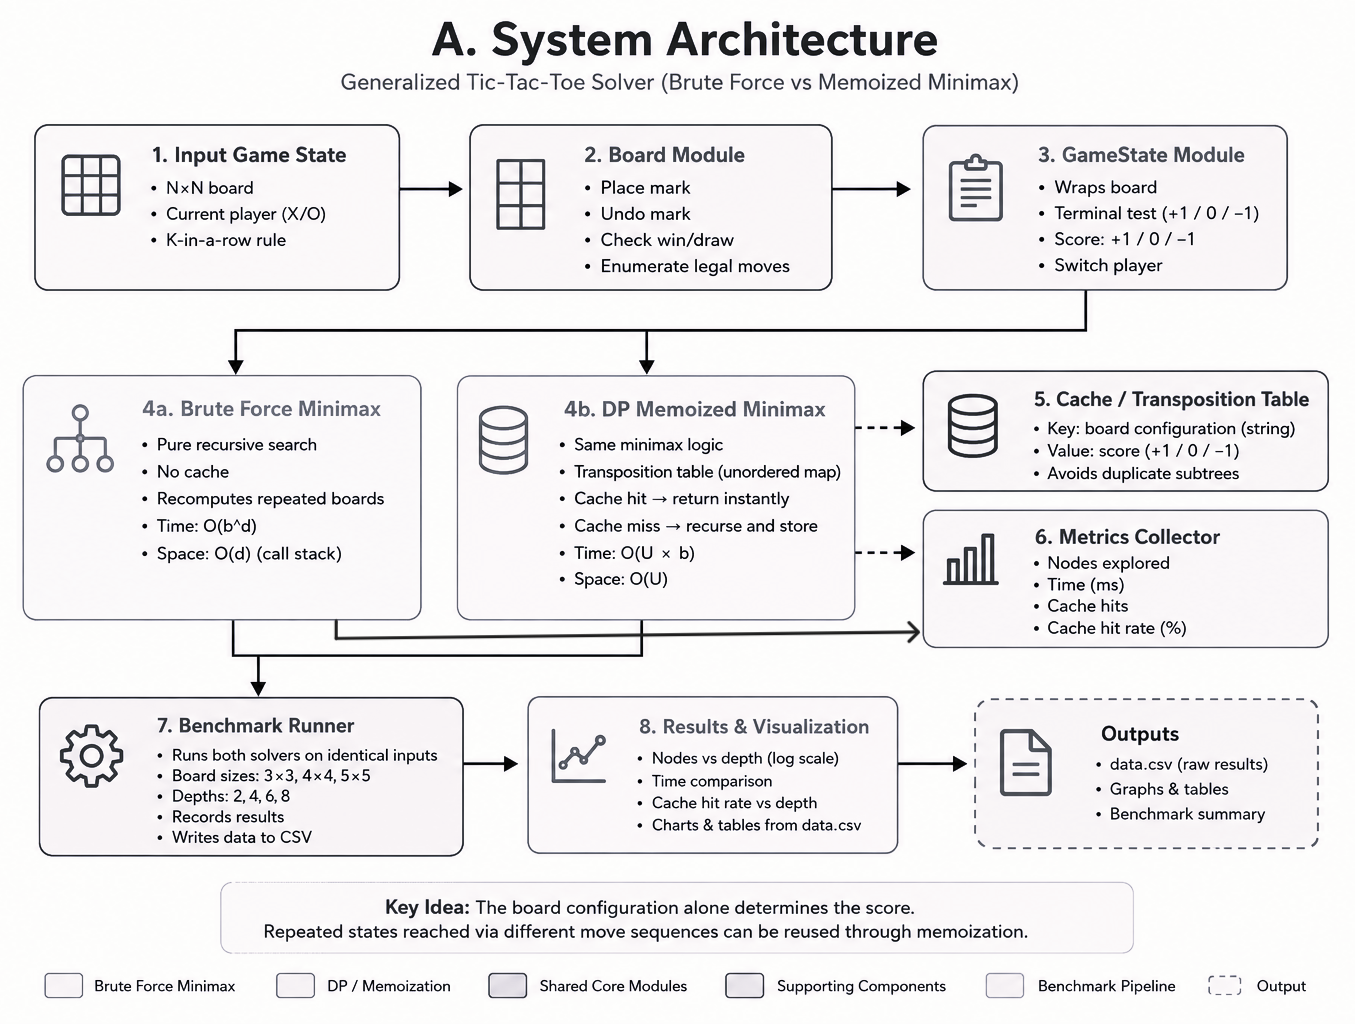
\includegraphics[width=\columnwidth]{XO-Dia1.png}
\caption{System architecture: the benchmark selects a solver and
collects performance metrics. The DP solver additionally tracks
cache hits.}
\label{fig:architecture}
\end{figure}

\subsection{Benchmarking Setup}
All experiments run on a 3.0 GHz CPU with 16 GB RAM, compiled with
\texttt{g++ -O3}. The parameter grid is:
\begin{itemize}
    \item Board sizes: $N \in \{3, 4, 5\}$
    \item Search depths: $d \in \{2, 4, 6, 8\}$
    \item Win length $K = N$ (standard Tic-Tac-Toe)
\end{itemize}
Each configuration plays a full game; at each ply the solver is called,
its metrics are reset, and results are summed across the game. Timeouts
are rule-based: brute force is skipped for $4\times4, d\ge 8$ and
$5\times5, d\ge 6$, while DP is skipped for $5\times5, d\ge 8$.

% ─────────────────────────────────────────────────────────────────
\subsection{Brute-Force Minimax Solver}
% ─────────────────────────────────────────────────────────────────
The brute-force Minimax algorithm computes the optimal move through
exhaustive recursive exploration of every possible game state~\cite{b3}.
At every position, all legal moves are tried; the maximizer keeps the
highest resulting score and the minimizer keeps the lowest. No result is
stored: if the same board appears via two distinct move sequences, the
entire subtree beneath it is recomputed from scratch both times~\cite{b4}.

\subsubsection{Approach}
The brute-force method employs a pure recursive backtracking algorithm
that tests all possible continuations from the current position. The
algorithm maintains a shared \texttt{Board} object, mutating it in place
via \texttt{placeMark} and restoring it via \texttt{undoMark} after each
recursive call, to avoid copying the grid at every node.

Key components of the approach include:
\begin{itemize}
    \item \textbf{State Representation}: An $N \times N$ grid of
    \texttt{Cell} enumerations (\texttt{EMPTY}, \texttt{X}, \texttt{O})
    wrapped in a \texttt{GameState} object that also tracks the current
    player.
    \item \textbf{Move Generation}: At each node,
    \texttt{getEmptyCells()} returns all unoccupied positions as legal
    moves.
    \item \textbf{Terminal Detection}: \texttt{isTerminal()} returns
    true when a player achieves $K$ in a row or the board is full;
    \texttt{getScore()} returns $+1$, $-1$, or $0$.
    \item \textbf{Undo-Move Pattern}: After returning from a recursive
    call, \texttt{undoMark} and \texttt{switchPlayer} restore the shared
    state, reducing per-node overhead to $O(1)$.
\end{itemize}

Starting from the current board, the algorithm tries every legal move,
recurses into the resulting position, and picks the best score for the
current player.

\subsubsection{The Algorithm}
The implementation consists of two functions working together to evaluate
the entire reachable game tree.

\textbf{Function Signatures:}

\begin{algorithm}[htbp]
\caption{Function Signatures (Brute-Force)}
\begin{algorithmic}[1]
\Procedure{getBestMove}{$state$}
\State {$state$: the current \texttt{GameState} (board + current player)}
\State \textbf{returns}: the optimal \texttt{Move} $\{row, col\}$
\EndProcedure
\Procedure{minimax}{$state, depth, isMaximizing$}
\State {$state$: shared mutable \texttt{GameState}}
\State {$depth$: remaining search depth}
\State {$isMaximizing$: \textbf{true} if X's turn, \textbf{false} if O's turn}
\State \textbf{returns}: integer Minimax score for the current position
\EndProcedure
\end{algorithmic}
\end{algorithm}

\textbf{Node Counter:}
Every call to \texttt{minimax} increments the node counter.

\begin{algorithm}[htbp]
\caption{Node Counter}
\begin{algorithmic}[1]
\State $metrics.nodesExplored \gets metrics.nodesExplored + 1$
\end{algorithmic}
\end{algorithm}

\textbf{Base Cases:}
Terminal positions are scored immediately; depth limit returns $0$.

\begin{algorithm}[htbp]
\caption{Base Cases}
\begin{algorithmic}[1]
\If{$state.isTerminal()$}
    \State \Return $state.getScore()$
    \Comment{$+1$ (X wins), $-1$ (O wins), or $0$ (draw)}
\EndIf
\If{$depth = 0$}
    \State \Return $0$
    \Comment{Depth limit reached; no heuristic}
\EndIf
\end{algorithmic}
\end{algorithm}

\textbf{Move Generation:}
All legal moves are collected from the current board.

\begin{algorithm}[htbp]
\caption{Move Generation}
\begin{algorithmic}[1]
\State $moves \gets state.board.getEmptyCells()$
\State \Comment{Returns \texttt{vector<Move>} of all $\{row, col\}$ pairs where
\texttt{grid[row][col] = EMPTY}}
\end{algorithmic}
\end{algorithm}

\textbf{Maximizer and Minimizer Branches:}

\begin{algorithm}[htbp]
\caption{Maximizer and Minimizer Branches}
\begin{algorithmic}[1]
\If{$isMaximizing$}
    \State $best \gets -\infty$
    \For{each $m \in moves$}
        \State $state.board.placeMark(m)$; \quad $state.switchPlayer()$
        \State $val \gets \Call{minimax}{state,\; depth-1,\; \textbf{false}}$
        \State $state.switchPlayer()$; \quad $state.board.undoMark(m)$
        \State $best \gets \max(best, val)$
    \EndFor
\Else
    \State $best \gets +\infty$
    \For{each $m \in moves$}
        \State $state.board.placeMark(m)$; \quad $state.switchPlayer()$
        \State $val \gets \Call{minimax}{state,\; depth-1,\; \textbf{true}}$
        \State $state.switchPlayer()$; \quad $state.board.undoMark(m)$
        \State $best \gets \min(best, val)$
    \EndFor
\EndIf
\State \Return $best$
\end{algorithmic}
\end{algorithm}

\textbf{Entry Point --- getBestMove:}

\begin{algorithm}[htbp]
\caption{Entry Point: getBestMove}
\begin{algorithmic}[1]
\Procedure{getBestMove}{$state$}
    \State $start \gets \texttt{high\_resolution\_clock::now()}$
    \State $bestMove \gets \{-1,-1\}$
    \State $bestScore \gets -\infty$ \textbf{ if } X's turn, \textbf{ else } $+\infty$
    \For{each $m \in state.board.getEmptyCells()$}
        \State $state.board.placeMark(m)$; \quad $state.switchPlayer()$
        \State $score \gets \Call{minimax}{state,\; maxDepth - 1,\; \neg isMaximizing}$
        \State $state.switchPlayer()$; \quad $state.board.undoMark(m)$
        \If{$score$ improves $bestScore$}
            \State $bestScore \gets score$; \quad $bestMove \gets m$
        \EndIf
    \EndFor
    \State $metrics.timeMs \gets$ elapsed milliseconds
    \State \Return $bestMove$
\EndProcedure
\end{algorithmic}
\end{algorithm}

\subsubsection{Complexity Analysis}
\textbf{Time Complexity:} Starting from an empty $N \times N$ board, the
first move has $N^2$ options, the second $N^2 - 1$, and so on. The total
nodes explored up to depth $d$ is bounded by
$\prod_{i=0}^{d-1}(N^2 - i) \leq (N^2)^d$, giving $O(b^d)$ where
$b = N^2$ is the branching factor. For $N = 5$ and $d = 8$ this yields
an upper bound of $25^8 \approx 1.5 \times 10^{11}$ nodes.

\textbf{Space Complexity:} The algorithm uses $O(d)$ space for the
recursion call stack. The shared board occupies $O(N^2)$ space that is
mutated in place and does not grow with depth. No additional storage
is allocated.

\subsubsection{Step-by-Step Trace for a Near-Terminal $3 \times 3$ Position}
To illustrate the process, consider the following position with O
(Minimizer) to move at depth $d = 2$:

\begin{center}
\setlength{\tabcolsep}{8pt}
\renewcommand{\arraystretch}{1.3}
\begin{tabular}{c|c|c}
X & \_ & X \\ \hline
O & O & \_ \\ \hline
\_ & \_ & \_ \\
\end{tabular}
\end{center}

O can win immediately by playing at position $(1,2)$, completing row~1.

\begin{table}[htbp]
\centering
\caption{Brute-force execution trace ($3 \times 3$, O to move, $d=2$)}
\label{tab:bf_trace}
\renewcommand{\arraystretch}{2.0}
\begin{tabular}{|p{0.5cm}|p{2.5cm}|p{1.5cm}|p{2.2cm}|}
\hline
\textbf{Step} & \textbf{Action} & \textbf{Move} & \textbf{Result} \\
\hline
1 & Root: O (Minimizer), 5 empty cells & --- & $best = +\infty$ \\
\hline
2 & Try O$\to$(0,1), recurse to $d{=}1$ & (0,1) & No win; score $= 0$ \\
\hline
3 & Try O$\to$(1,2), check terminal & (1,2) & O wins! score $= -1$ \\
\hline
4 & $-1 < +\infty$, update $best$ & --- & $bestMove = (1,2)$ \\
\hline
5 & Try remaining 3 moves & ... & All scores $\geq -1$ \\
\hline
6 & Return best move & (1,2) & Score $= -1$ (O wins) \\
\hline
\end{tabular}
\end{table}

\textit{Note: The brute-force solver recomputes every subtree
independently, even if an identical board has already been evaluated via
a different sequence of moves.}

% ─────────────────────────────────────────────────────────────────
\subsection{DP Memoized Minimax Solver}
% ─────────────────────────────────────────────────────────────────
The DP memoized Minimax algorithm applies the same Minimax recurrence as
the brute-force solver but adds a transposition table: a hash map from
board configuration (plus remaining depth) to its precomputed Minimax
score~\cite{b4, b5}. The key observation exploited is that different move
sequences can produce the same board configuration, and the Minimax value
of that configuration depends only on the board and the remaining
depth---not on the path taken to reach it. This is the overlapping
subproblems property that makes dynamic programming applicable~\cite{b4}.

The transposition table is implemented as a \texttt{Cache} class wrapping
an \texttt{std::unordered\_map<std::string,\,int>}. On the first
encounter of a configuration, its score is computed normally and stored
in the table. On any subsequent encounter, the stored score is returned
in $O(1)$, and the entire subtree beneath that node is skipped entirely.

\subsubsection{Approach}
The memoized approach uses the same recursive backtracking structure as
the brute-force solver---including the undo-move pattern---with one
structural addition: a cache lookup at the top of each recursive call
and a cache write before every return.

Key components of the approach include:
\begin{itemize}
    \item \textbf{Cache Key}: The board is serialized row-major into a
    string of \texttt{'X'}, \texttt{'O'}, and \texttt{'\_'} characters
    by \texttt{board.getKey()}, then the remaining depth is appended.
    Including depth is critical: the same board evaluated at $d = 2$ may
    score differently than at $d = 6$, since the deeper search detects
    wins that the shallower one cannot.
    \item \textbf{Cache Lookup}: Before any recursive work,
    \texttt{cache.get(key)} returns a \texttt{std::optional<int>}.
    A hit increments \texttt{cacheHits} and returns immediately; a miss
    proceeds with normal computation.
    \item \textbf{Cache Write}: Every computed score is stored before
    returning, so the first computation of any state is the last.
    \item \textbf{Cache Invalidation}: \texttt{cache.clear()} is called
    inside \texttt{resetMetrics()} between benchmark runs, preventing
    stale entries from crossing run boundaries.
\end{itemize}

\subsubsection{The Algorithm}
The implementation mirrors the brute-force structure with three additions:
key construction, cache lookup, and cache write.

\textbf{Function Signature:}

\begin{algorithm}[htbp]
\caption{Function Signature (DP Memoized)}
\begin{algorithmic}[1]
\Procedure{MinimaxDP}{$state, depth, isMaximizing$}
\State {$state$: shared mutable \texttt{GameState}}
\State {$depth$: remaining search depth}
\State {$isMaximizing$: \textbf{true} for X (maximizer), \textbf{false} for O (minimizer)}
\State \textbf{returns}: integer Minimax score, looked up or computed
\EndProcedure
\end{algorithmic}
\end{algorithm}

\textbf{Cache Key Construction:}

\begin{algorithm}[htbp]
\caption{Cache Key Construction}
\begin{algorithmic}[1]
\State $key \gets state.board.getKey()$
    \texttt{ + "|" + } $\texttt{to\_string}(depth)$
\State \Comment{\texttt{getKey()} returns a string such as
    \texttt{"X\_XOO\_\_\_\_"} for a $3{\times}3$ grid}
\State \Comment{The depth suffix distinguishes the same board at
    different search horizons}
\end{algorithmic}
\end{algorithm}

\textbf{Cache Lookup:}

\begin{algorithm}[htbp]
\caption{Cache Lookup}
\begin{algorithmic}[1]
\State $metrics.nodesExplored \gets metrics.nodesExplored + 1$
\If{$cache.get(key) \neq \texttt{nullopt}$}
    \State $metrics.cacheHits \gets metrics.cacheHits + 1$
    \State \Return $cache.get(key)$
    \Comment{$O(1)$ --- entire subtree is skipped}
\EndIf
\end{algorithmic}
\end{algorithm}

\textbf{Base Cases with Cache Write:}

\begin{algorithm}[htbp]
\caption{Base Cases with Cache Write}
\begin{algorithmic}[1]
\If{$state.isTerminal()$}
    \State $score \gets state.getScore()$
    \State $cache.set(key, score)$
    \State \Return $score$
\EndIf
\If{$depth = 0$}
    \State $cache.set(key, 0)$; \quad \Return $0$
\EndIf
\end{algorithmic}
\end{algorithm}

\textbf{Recursive Core with Final Cache Write:}

\begin{algorithm}[htbp]
\caption{Recursive Core with Cache Write}
\begin{algorithmic}[1]
\State $moves \gets state.board.getEmptyCells()$
\State $score \gets -\infty$ \textbf{ if } $isMaximizing$ \textbf{ else } $+\infty$
\For{each $m \in moves$}
    \State $state.board.placeMark(m)$; \quad $state.switchPlayer()$
    \State $val \gets \Call{MinimaxDP}{state,\; depth-1,\; \neg isMaximizing}$
    \State $state.switchPlayer()$; \quad $state.board.undoMark(m)$
    \If{$isMaximizing$}
        \State $score \gets \max(score, val)$
    \Else
        \State $score \gets \min(score, val)$
    \EndIf
\EndFor
\State $cache.set(key, score)$
\Comment{Store result; converts every future visit to $O(1)$}
\State \Return $score$
\end{algorithmic}
\end{algorithm}

\subsubsection{Complexity Analysis}
\textbf{Time Complexity:} Let $U$ be the number of unique board
configurations reachable from the initial state within depth $d$. Each
unique state is computed at most once per depth level, performing $O(b)$
work per state. Total complexity is therefore $O(U \cdot b)$, where
$U \ll b^d$ because many distinct move sequences converge to the same
configuration. In practice, cache hit rates of 49--73.6\% are observed
(Table~\ref{tab:cachehit}), confirming that the majority of recursive
calls are served from cache at sufficient depth.

\textbf{Space Complexity:} The algorithm requires $O(U)$ space for the
transposition table and $O(d)$ for the call stack. The cache grows
monotonically during a single search and is cleared by
\texttt{resetMetrics()} between runs.

\subsubsection{Step-by-Step Trace Showing Cache Behavior}
Using the same near-terminal $3 \times 3$ position, with O to move at
$d = 2$, the following trace shows how the transposition table eliminates
redundant computation when the same board is reached via two different
parent paths.

\begin{table}[htbp]
\centering
\caption{DP memoized trace: cache hit eliminates subtree recomputation}
\label{tab:dp_trace}
\renewcommand{\arraystretch}{2.0}
\begin{tabular}{|p{0.5cm}|p{2.3cm}|p{1.0cm}|p{2.7cm}|}
\hline
\textbf{Step} & \textbf{Board Key} & \textbf{Cache} & \textbf{Action / Result} \\
\hline
1 & \texttt{"X\_XOO\_\_\_\_|2"} & Miss & Compute; explore all 5 O moves \\
\hline
2 & \texttt{"X\_XOOO\_\_\_|1"} & Miss & O wins; $score{=}{-1}$; store in cache \\
\hline
3 & \texttt{"X\_XOO\_\_\_\_|2"} & --- & $best{=}{-1}$, $bestMove{=}(1,2)$ \\
\hline
4 & \texttt{"X\_XOOO\_\_\_|1"} & \textbf{Hit!} & Same state via alternate path \\
\hline
5 & --- & --- & Return $-1$ instantly; subtree skipped \\
\hline
6 & Final answer & --- & $bestMove{=}(1,2)$, score ${= -1}$ \\
\hline
\end{tabular}
\end{table}

\textit{Note: Step 4 is the cache hit. The state produced by O playing
(1,2) through a different parent branch is found in the table and
returned in $O(1)$, avoiding full recomputation of its subtree.}

% ─────────────────────────────────────────────────────────────────
% 8. RESULTS AND EVALUATION
% ─────────────────────────────────────────────────────────────────
\section{Results and Evaluation}

Both methods correctly compute the optimal Minimax move from any given
position; they differ fundamentally in how they handle repeated board
configurations across the search tree~\cite{b3, b4}.

\subsection{Performance Comparison}
Table~\ref{tab:comparison} summarizes their algorithmic characteristics.

\begin{table}[htbp]
\centering
\caption{Algorithmic Characteristics Comparison}
\label{tab:comparison}
\renewcommand{\arraystretch}{1.6}
\begin{tabular}{|p{2.2cm}|p{2.0cm}|p{2.0cm}|}
\hline
\textbf{Aspect} & \textbf{Brute Force} & \textbf{DP Memoized} \\
\hline
Time Complexity & $O(b^d)$ & $O(U \cdot b)$ \\
\hline
Space Complexity & $O(d)$ & $O(U + d)$ \\
\hline
Cache & None & \texttt{unordered\_map} \\
\hline
Repeated State & Full recomputation & $O(1)$ lookup \\
\hline
Configs Completed & 9 of 12 & 11 of 12 \\
\hline
\end{tabular}
\end{table}

Table~\ref{tab:cachehit} reports the DP solver’s cache hit rates. The
hit rate grows from 0\% at $d=2$ to 73.6\% at $4\times4, d=8$, illustrating
the increasing density of transpositions deeper in the tree.

\begin{table}[htbp]
\centering
\caption{DP Memoized Solver: Nodes Explored and Cache Hit Rate}
\label{tab:cachehit}
\renewcommand{\arraystretch}{1.6}
\begin{tabular}{|p{1.4cm}|p{0.7cm}|p{1.5cm}|p{1.3cm}|p{1.2cm}|}
\hline
\textbf{Board} & \textbf{Depth} & \textbf{Nodes} &
\textbf{Cache Hits} & \textbf{Hit Rate} \\
\hline
$3{\times}3$ & 2 &       276 &         0 & 0.0\% \\
\hline
$3{\times}3$ & 4 &     4,481 &     2,094 & 46.7\% \\
\hline
$3{\times}3$ & 6 &    16,449 &     9,968 & 60.6\% \\
\hline
$3{\times}3$ & 8 &    22,690 &    14,455 & 63.7\% \\
\hline
$4{\times}4$ & 2 &     1,496 &         0 & 0.0\% \\
\hline
$4{\times}4$ & 4 &    89,734 &    44,093 & 49.1\% \\
\hline
$4{\times}4$ & 6 & 1,620,848 & 1,064,327 & 65.7\% \\
\hline
$4{\times}4$ & 8 & 11,707,893 & 8,621,896 & 73.6\% \\
\hline
$5{\times}5$ & 2 &     5,525 &         0 & 0.0\% \\
\hline
$5{\times}5$ & 4 &   884,190 &   439,280 & 49.7\% \\
\hline
$5{\times}5$ & 6 & 47,247,018 & 31,346,686 & 66.4\% \\
\hline
\end{tabular}
\end{table}

At $N = 3$, $d = 8$, both solvers complete: brute force explores
490,303 nodes in 407.06\,ms, while DP explores 22,690 nodes in
24.97\,ms, a $21.6{\times}$ node reduction. At $N = 4$, $d = 6$, brute
force explores 15,577,978 nodes in 7,291.3\,ms, while DP explores
1,620,848 nodes in 1,142.19\,ms with a 65.7\% hit rate. At $N = 4$,
$d = 8$, DP explores 11,707,893 nodes with a 73.6\% hit rate and
finishes in 9,518.55\,ms, while brute force is skipped by the timeout
rule. At $N = 5$, $d = 6$, DP completes in 55,221.8\,ms with 66.4\%
cache hits, while brute force is skipped.

\subsection{Strengths and Limitations}
\textbf{Brute Force Approach:}
\textit{Strengths:} conceptually simple, minimal memory ($O(d)$), no
cache concerns.
\textit{Limitations:} exponential time; recomputes every transposed
position; skipped by timeout rules at $4\times4, d\ge 8$ and
$5\times5, d\ge 6$.

\textbf{DP Memoized Approach:}
\textit{Strengths:} eliminates redundant subtree computation; cache hit
rate grows with depth (up to 73.6\%); handles $N=5, d=6$.
\textit{Limitations:} memory grows as $O(U)$; string‑key overhead; no
benefit at very shallow depths.

% ─────────────────────────────────────────────────────────────────
% 9. DISCUSSION
% ─────────────────────────────────────────────────────────────────
\section{Discussion}

The results clearly demonstrate that brute-force Minimax scales
exponentially and becomes impractical beyond the largest configurations
allowed by the timeout rules, while the DP memoized solver handles
significantly larger instances by reusing computations. The cache hit
rate is the critical factor: at $d=2$ (0\% hits) both solvers behave
similarly; as depth increases, the hit rate reaches 73.6\%, reducing the
effective node count by a factor of $1/(1-\text{hit rate})$. For
$N=4, d=8$, the memoized solver explores 11.7M nodes but avoids
8.6M recomputations, yielding a feasible search where brute force is
skipped.

The memoized approach does incur a string‑key overhead and uses
substantial memory. Nevertheless, for any non‑trivial depth, the trade‑off
is overwhelmingly favorable. The brute-force implementation remains
valuable as a pedagogic baseline and a correctness reference.

% ─────────────────────────────────────────────────────────────────
% 10. CONCLUSION
% ─────────────────────────────────────────────────────────────────
\section{Conclusion}

This paper presented a direct comparison of brute-force and DP memoized
Minimax algorithms for solving the generalized Tic‑Tac‑Toe problem.
The DP solver exploits overlapping subproblems to achieve dramatic
reductions in search space, completing 11 of 12 benchmark configurations
while brute force completes 9 of 12. The cache hit rate, reaching
73.6\% at $d=8$, quantifies the benefit of memoization. The work
underscores the importance of dynamic programming techniques in
adversarial search and provides a clear, measurable case study suitable
for AI education and algorithm design.

% ─────────────────────────────────────────────────────────────────
% 11. FUTURE WORK
% ─────────────────────────────────────────────────────────────────
\section{Future Work}

Several enhancements can be explored:
\begin{itemize}
    \item Incorporate alpha‑beta pruning into both solvers to further
          reduce the effective branching factor.
    \item Replace the depth‑limited neutral heuristic with a positional
          evaluation function to allow informed play at any depth.
    \item Implement iterative deepening and time‑limited search for
          real‑time applications.
    \item Apply the same benchmarking methodology to other combinatorial
          games (e.g., Connect‑Four, Othello) to generalize the findings.
    \item Investigate more memory‑efficient caching strategies, such as
          LRU eviction, to limit memory usage in very deep searches.
\end{itemize}

% ─────────────────────────────────────────────────────────────────
% 12. REFERENCES (IEEE Style)
% ─────────────────────────────────────────────────────────────────
\begin{thebibliography}{00}
\bibitem{b1} S. J. Russell and P. Norvig, ``Artificial Intelligence:
A Modern Approach,'' 4th ed., Pearson, 2020.
\bibitem{b2} C. E. Shannon, ``Programming a computer for playing chess,''
\textit{Philosophical Magazine}, vol. 41, no. 314, pp. 256--275, 1950.
\bibitem{b3} D. E. Knuth and R. W. Moore, ``An analysis of alpha-beta
pruning,'' \textit{Artificial Intelligence}, vol. 6, no. 4,
pp. 293--326, 1975.
\bibitem{b4} T. H. Cormen, C. E. Leiserson, R. L. Rivest, and C. Stein,
``Introduction to Algorithms,'' 4th ed., MIT Press, 2022.
\bibitem{b5} A. L. Zobrist, ``A new hashing method with application for
game playing,'' Technical Report 88, Univ. of Wisconsin, 1970.
\bibitem{b6} S. S. Skiena, ``The Algorithm Design Manual,'' 2nd ed.,
Springer, 2008.
\end{thebibliography}

\end{document}